\section{Lundi 14 septembre 2020}

Pllanche de TD 1.

\subsection{Exercice 1}

Quelques rappels :

\begin{itemize}
\tightlist
	\item Un signal numérique ou en bande de bases est à valeur discrètes.
	\item Un signal analogique peut prendre n'importe quelle valeur dans un intervalle.
	\item Un modem convertit d'un signal analogique vers un signal numérique et inversement.
	\item Sur un signal analogique, on note $T$ la période, et $\frac{1}{T}$ la fréquence
\end{itemize}

Questions :

\begin{enumerate}
\tightlist

	\item Des connexions qui permettent le dialogue bidirectionnel à l'alternat sont connues comme \textbf{half duplex}.
	\item Une transmission en bande de base correspond à une transmission \textbf{numérique}.
	\item L'interconnexion de machine par l'intermédiaire d'un Hub correspond à une topologie en \textbf{bus}.
	\item La taille du message reçu par la couche 3 de la machine B est \textbf{60 octets}.

\end{enumerate}

\subsection{Exercice 2}

Questions :

\begin{enumerate}
	\item Les avantages sont par exemple la facilité de maintenance de chacune des couches, et l'interopérabilité entre les systèmes hétérogènes. Un inconvénient est la rigidité des normes utilisées.
	\item Des standards permettant l'interopérabilité sont par exemple les vis, les pneus de voitures ou les piles. Cette interopérabilité n'existe pas par exemple pour les chargeurs de téléphone, les prises électrique, ou les cartouches d'encre d'imprimante.
	\item La fibre a par exemple une bande passante élevée et une latence faible, alors que le wifi à un débit moyen et une latence élevée.
	\item Les deux cas sont différents. Un message est traité dans sa globalité pour traverser le réseau ; alors que pour un flot d'octets, le message est découpé en octets, traités de façon indépendantes les uns des autres.
	\item Si la norme est respectée, alors il ne devrait pas y avoir d'impact.
	\item
		\begin{tabular}[t]{|l|l|l|l|}
\hline
 & faible & moyen & long \\ \hline
étoile & 2 & 2 & 2 \\ \hline
double & 1 & $\frac{n}{4}$ & $\frac{n}{2}$ \\ \hline
maillage complet & 1 & 1 & 1 \\ \hline
\end{tabular}
\end{enumerate}

\subsection{Exercice 3}

Note : cet exercice n'a pas été corrigé en TD, ceci est juste mon brouillon.

Note : chaque bit affiché en dessous de chaque chronogramme est au milieu de l'intervalle de temps prévu à sa transmission.

\begin{figure}[H]
\centering
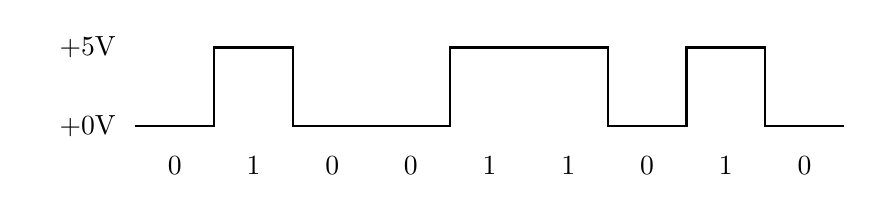
\begin{tikzpicture}
	\draw[thick,black] (0,0) -- (1,0) -- (1,1) -- (2,1) -- (2,0) -- (4,0) -- (4,1) -- (6,1) -- (6,0) -- (7,0) -- (7,1) -- (8,1) -- (8,0) -- (9,0);
	\node[text width=1cm, align=right] at (-.75,0) {+0V};
	\node[text width=1cm, align=right] at (-.75,1) {+5V};
	\node[text width=1cm, align=center] at (0.5,-.5) {0};
	\node[text width=1cm, align=center] at (1.5,-.5) {1};
	\node[text width=1cm, align=center] at (2.5,-.5) {0};
	\node[text width=1cm, align=center] at (3.5,-.5) {0};
	\node[text width=1cm, align=center] at (4.5,-.5) {1};
	\node[text width=1cm, align=center] at (5.5,-.5) {1};
	\node[text width=1cm, align=center] at (6.5,-.5) {0};
	\node[text width=1cm, align=center] at (7.5,-.5) {1};
	\node[text width=1cm, align=center] at (8.5,-.5) {0};
\end{tikzpicture}
\caption{Le code tout ou rien}
\end{figure}

\begin{figure}[H]
\centering
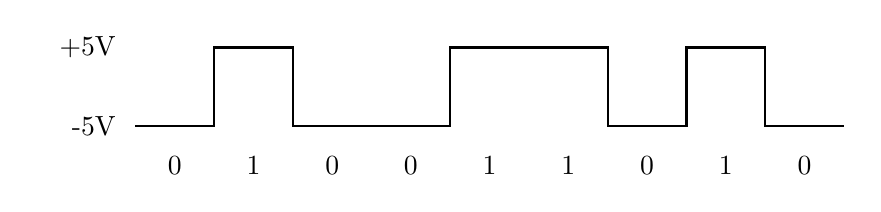
\begin{tikzpicture}
	\draw[thick,black] (0,0) -- (1,0) -- (1,1) -- (2,1) -- (2,0) -- (4,0) -- (4,1) -- (6,1) -- (6,0) -- (7,0) -- (7,1) -- (8,1) -- (8,0) -- (9,0);
	\node[text width=1cm, align=right] at (-.75,0) {-5V};
	\node[text width=1cm, align=right] at (-.75,1) {+5V};
	\node[text width=1cm, align=center] at (0.5,-.5) {0};
	\node[text width=1cm, align=center] at (1.5,-.5) {1};
	\node[text width=1cm, align=center] at (2.5,-.5) {0};
	\node[text width=1cm, align=center] at (3.5,-.5) {0};
	\node[text width=1cm, align=center] at (4.5,-.5) {1};
	\node[text width=1cm, align=center] at (5.5,-.5) {1};
	\node[text width=1cm, align=center] at (6.5,-.5) {0};
	\node[text width=1cm, align=center] at (7.5,-.5) {1};
	\node[text width=1cm, align=center] at (8.5,-.5) {0};
\end{tikzpicture}
\caption{Le code NRZ}
\end{figure}

\begin{figure}[H]
\centering
\begin{tikzpicture}
	\draw[thick,black] (0,1) -- (1,1) -- (1,2) -- (2,2) -- (2,1) -- (4,1) -- (4,0) -- (5,0) -- (5,2) -- (6,2) -- (6,1) -- (7,1) -- (7,0) -- (8,0) -- (8,1) -- (9,1);
	\node[text width=1cm, align=right] at (-.75,0) {-5V};
	\node[text width=1cm, align=right] at (-.75,1) {+0V};
	\node[text width=1cm, align=right] at (-.75,2) {+5V};
	\node[text width=1cm, align=center] at (0.5,-.5) {0};
	\node[text width=1cm, align=center] at (1.5,-.5) {1};
	\node[text width=1cm, align=center] at (2.5,-.5) {0};
	\node[text width=1cm, align=center] at (3.5,-.5) {0};
	\node[text width=1cm, align=center] at (4.5,-.5) {1};
	\node[text width=1cm, align=center] at (5.5,-.5) {1};
	\node[text width=1cm, align=center] at (6.5,-.5) {0};
	\node[text width=1cm, align=center] at (7.5,-.5) {1};
	\node[text width=1cm, align=center] at (8.5,-.5) {0};
\end{tikzpicture}
\caption{Le code bipolaire}
\end{figure}

\begin{figure}[H]
\centering
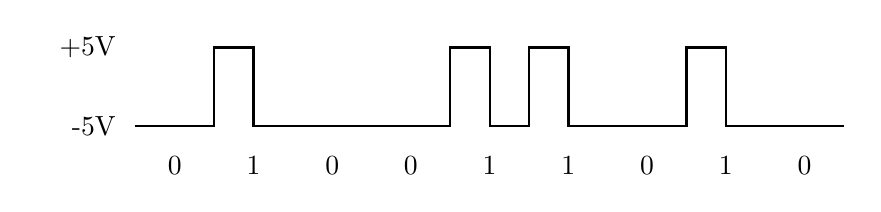
\begin{tikzpicture}
	\draw[thick,black] (0,0) -- (1,0) -- (1,1) -- (1.5,1) -- (1.5,0) -- (4,0) -- (4,1) -- (4.5,1) -- (4.5,0) -- (5,0) -- (5,1) -- (5.5,1) -- (5.5,0) -- (7,0) -- (7,1) -- (7.5,1) -- (7.5,0) -- (9,0);
	\node[text width=1cm, align=right] at (-.75,0) {-5V};
	\node[text width=1cm, align=right] at (-.75,1) {+5V};
	\node[text width=1cm, align=center] at (0.5,-.5) {0};
	\node[text width=1cm, align=center] at (1.5,-.5) {1};
	\node[text width=1cm, align=center] at (2.5,-.5) {0};
	\node[text width=1cm, align=center] at (3.5,-.5) {0};
	\node[text width=1cm, align=center] at (4.5,-.5) {1};
	\node[text width=1cm, align=center] at (5.5,-.5) {1};
	\node[text width=1cm, align=center] at (6.5,-.5) {0};
	\node[text width=1cm, align=center] at (7.5,-.5) {1};
	\node[text width=1cm, align=center] at (8.5,-.5) {0};
\end{tikzpicture}
\caption{Le code RZ}
\end{figure}


\begin{figure}[H]
\centering
\begin{tikzpicture}
	\draw[thick,black] (0,1) -- (1,1) -- (1,2) -- (2,2) -- (2,1) -- (4,1) -- (4,0) -- (5,0) -- (5,2) -- (6,2) -- (6,1) -- (7,1) -- (7,0) -- (8,0) -- (8,1) -- (9,1);
	\node[text width=1cm, align=right] at (-.75,0) {-5V};
	\node[text width=1cm, align=right] at (-.75,1) {+0V};
	\node[text width=1cm, align=right] at (-.75,2) {+5V};
	\node[text width=1cm, align=center] at (0.5,-.5) {0};
	\node[text width=1cm, align=center] at (1.5,-.5) {1};
	\node[text width=1cm, align=center] at (2.5,-.5) {0};
	\node[text width=1cm, align=center] at (3.5,-.5) {0};
	\node[text width=1cm, align=center] at (4.5,-.5) {1};
	\node[text width=1cm, align=center] at (5.5,-.5) {1};
	\node[text width=1cm, align=center] at (6.5,-.5) {0};
	\node[text width=1cm, align=center] at (7.5,-.5) {1};
	\node[text width=1cm, align=center] at (8.5,-.5) {0};
\end{tikzpicture}
\caption{Le code Manchester (NON FAIT)}
\end{figure}

\begin{figure}[H]
\centering
\begin{tikzpicture}
	\draw[thick,black] (0,1) -- (1,1) -- (1,2) -- (2,2) -- (2,1) -- (4,1) -- (4,0) -- (5,0) -- (5,2) -- (6,2) -- (6,1) -- (7,1) -- (7,0) -- (8,0) -- (8,1) -- (9,1);
	\node[text width=1cm, align=right] at (-.75,0) {-5V};
	\node[text width=1cm, align=right] at (-.75,1) {+0V};
	\node[text width=1cm, align=right] at (-.75,2) {+5V};
	\node[text width=1cm, align=center] at (0.5,-.5) {0};
	\node[text width=1cm, align=center] at (1.5,-.5) {1};
	\node[text width=1cm, align=center] at (2.5,-.5) {0};
	\node[text width=1cm, align=center] at (3.5,-.5) {0};
	\node[text width=1cm, align=center] at (4.5,-.5) {1};
	\node[text width=1cm, align=center] at (5.5,-.5) {1};
	\node[text width=1cm, align=center] at (6.5,-.5) {0};
	\node[text width=1cm, align=center] at (7.5,-.5) {1};
	\node[text width=1cm, align=center] at (8.5,-.5) {0};
\end{tikzpicture}
\caption{Le code Miller (NON FAIT)}
\end{figure}

